\documentclass{article}
\usepackage[utf8]{inputenc}
\usepackage{biblatex}
\usepackage{hyperref}
\usepackage{graphicx}


\addbibresource{bibliography.bib}

\title{Pokémon\textsuperscript{\small TM} and Reinforcement Learning\\ \large Project for Advanced Intelligent Systems course at Unimi}
\author{Dell'Acqua Matteo 09488A}
\date{\today}
\renewcommand*\contentsname{Summary}

\begin{document}

\maketitle
\newpage
\tableofcontents
\newpage

%\chapter{The uni project}

\section{Introduction}

The objective of this project is to create an agent capable of learning how to play Pokémon without any prior knowledge and without complex actions (every possible action in the environment is available to the agent directly).
A first experiment is created without using neural networks to show how the complex environment of a Pokémon battle cannot be modeled by a simple Q-table (which has no generalization capabilities).
The second experiment uses a neural network and provides far better results, though still far from being usable against a human player that more or less knows how to play.

\section{The Problem}

A \textbf{Pokémon\textsuperscript{\tiny TM}} match is an extremely complex environment and training an agent in such an environment is no easy feat. The complexity is caused by different factors:
\begin{itemize}
    \item it is a stochastic game;
    \item it is a game with incomplete information;
    \item the state of the environment is characterized by a large number of variables.
\end{itemize}

\subsection{Randomness in Pokémon}

To an external observer Pokémon may seem deterministic, and while they would be largely correct, the game is in fact stochastic. This non-determinism is caused by different components but it is all linked to attacks and damage calculation.

\subsubsection{Accuracy check}

Even before entering the damage calculation, a first roll of the dice is to determine whether the move will hit or miss. Every move has an \textbf{accuracy} value between 0 and 100 (representing hit percentage). There are also moves that skip the accuracy check (always or under certain conditions).
If the check succeeds the damage calculation starts.

\subsubsection{Damage calculation}

The damage calculation part of an attack is handled by the following formula \cite{Damage} (stochastic parts in bold):

\begin{equation}
    Damage = Stats \; multiplier \times Battle \; multiplier \times \textbf{Stochastic multiplier}
\end{equation}

in particular with:

\begin{equation}
    Stats \; multiplier = \left(\frac{\left(\frac{2 \times Level}{5} + 2\right) \times Power \times \frac{A}{D}}{50} + 2 \right) \times Type
\end{equation}

where

\begin{itemize}
    \item $Level$ is the level of the attacking Pokémon (between 1 and 100);
    \item $Power$ is the base power of the move;
    \item $A$ is the relative statistic of the attacking Pokémon (Attack if the move is physical, Special Attack if the move is special);
    \item $D$ is the relative statistic of the defending Pokémon (Defense if the move is physical, Special Defense if the move is special);
    \item $Type$ is the type effectiveness. This can be 0.25, 0.5 (not very effective), 1.0 (normally effective), 2.0 or 4.0 (supereffective), depending on both the move's and the target's types.
\end{itemize}

\begin{equation}
    Battle \; multiplier = Targets \times PB \times Weather \times STAB \times Burn \times Other \times ZMove
\end{equation}

where

\begin{itemize}
    \item $Targets$ is 0.75 (0.5 in Battle Royals) if the move has more than one target when the move is executed, 1.0 otherwise;
    \item $PB$ is 0.25 (0.5 in Generation VI) if the move is the second strike of Parental Bond, and 1.0 otherwise;
    \item $Weather$ is the multiplier based on the current weather;
    \item $STAB$ is the same-type attack bonus. This is equal to 1.5 if the move's type matches any of the user's types, 1.0 otherwise ;
    \item $Burn$ is 0.5 if the attacker is burned, its Ability is not Guts, and the used move is a physical move (other than Facade from Generation VI onward), 1.0 otherwise;
    \item $Other$ is 1.0 in most cases, and a different multiplier when specific interactions of moves, Abilities, or items take effect. If multiple effects influence the other value, their values stack multiplicatively;
    \item $ZMove$ is a multiplier for moves that get reduced but not stopped by protect-like moves. In case it reduces the damage, its value is 0.25, 1.0 otherwise.
\end{itemize}

\begin{equation}
    Stochastic \; multiplier = \textbf{Critical} \times \textbf{Random}
\end{equation}

where

\begin{itemize}
    \item $\textbf{Critical}$ is 1.5 (2 in Generation V) for a critical hit, 1 otherwise. This is stochastic;
    \item $\textbf{Random}$ is a random factor between 0.85 (low roll) and 1.0 (high roll).
\end{itemize}

\subsubsection{Optional side effects}

Every move may also have side effects on the defender and/or the attacker, like raising or lowering stats, inflicting status conditions, etc.
These are computed after the damage calculation, each with its own probability.

\subsubsection{Status conditions}
Conditions like confusion, sleep, freeze and paralysis heavily rely on randomness.
In particular, confusion and paralysis add an additional roll to the accuracy check. If it fails, the Pokémon won't be able to move (paralysis) or hit itself (confusion).
In the case of sleep, confusion and freeze, their duration also relies on randomness.

\subsection{Information in Pokémon}

Pokémon is a game with incomplete information, which means that an agent does not have the full information about the environment.
In particular, on the first turn it has access to full information regarding its own team, but only limited information about the opponent (only which Pokémon the opponent has deployed and sometimes its ability).
As the battle progresses, more information is available to the agent, like the opponent team when he chooses to switch out his Pokémon, or his team's moves when he uses one.
Regardless, it is highly unlikely for a game of Pokémon to ever reach a point where all the information is available to all the players.

\subsection{Variables in Pokémon}

A Pokémon battle is an extremely complex environment.
Even a simple single battle (each player can have at most 1 active Pokémon) has a really high number of variables.
For this project only single battles with 6 Pokémons for each player are considered.

\subsubsection{The team}

Each player has a team of 6 Pokémons.

\subsubsection{Pokémon}

Each Pokèmon is defined by a set of variables (not exaustive):
\begin{itemize}
    \item the base stats: 6 integers in [0, 255] defined by the species;
    \item the types: 1 or 2 types defined by the species. Used in damage multiplier calculation;
    \item the ability: defined by the species. Adds special effects to the Pokémon;
    \item the item: can be held by the Pokémon to add an additional effect;
    \item the moves: at most 4 moves. The species defines what moves can be learned;
    \item the possible mega evolution, which causes the ability and the base stats to change.
\end{itemize}
The Pokémon species is actually irrelevant.
It is better to use information defined by the species rather than using the species directly.

\subsubsection{Move}

Each move is defined by:
\begin{itemize}
    \item the base power;
    \item the accuracy;
    \item the type;
    \item the number of hits (most moves hit 1 time);
    \item additional effects (with randomness).
\end{itemize}

\section{Implementation}

The project is implemented in Python 3 and available on Github\cite{repo}.
In order to communicate with the \textit{Pokèmon Showdown} server\cite{smogon} the python package \textit{poke-env}\cite{pokeenv} is used.
For the neural network implementation, Tensorflow\cite{tensorflow} and TF-Agents\cite{TFAgents} are used.

\section{First solution: Q-Learning} \label{sarsa_results}

The first implemented solution tries to have an agent learn how to play Pokémon without using neural networks, leveraging only the Q-Learning algorithm against a state-action table.
In order to do this the observation space has to be reduced.

\subsection{Observation space}

The observation space tuple includes:
\begin{itemize}
    \item stats balance;
    \item damage multiplier balance;
    \item boosts balance;
    \item dynamaxed flag;
    \item forced switch flag;
    \item move value for every move.
\end{itemize}

\subsubsection{Stats balance}

\textbf{Stats balance} is an integer in [-2, 2].
It represents the balance of base stats between the agent's Pokémon and the enemy one.

\subsubsection{Damage multiplier balance}

\textbf{Damage multiplier} is an integer in [-1, 1].
It represents the balance of types between the agent's Pokémon and the enemy one.

\subsubsection{Boosts balance}

\textbf{Boosts balance} is an integer in [-1, 1].
It represents the balance of stat boosts between the agent's Pokémon and the enemy one.

\subsubsection{Dynamaxed}

\textbf{Dynamaxed} is a boolean flag that indicates whether the agent's Pokémon is dynamaxed.

\subsubsection{Forced switch}

\textbf{Forced switch} is a boolean flag that indicates whether the agent has to perform a switch.

\subsubsection{Move value}

Each move has a \textbf{move value}: an integer in [-7, 3].
It represents the value of the move in context of the battle based on the type of the move, the base power and the stat boosts.

\subsection{Action space} \label{action_space}

The action space includes all possible actions an agent can take in a turn.
In the case of a single battle, an action is represented by an integer in [0, 20].
In particular it uses:
\begin{itemize}
    \item {[0, 3]}: use the $i^{th}$ move;
    \item {[4, 7]}: use the $(i - 4)^{th}$ move as a \textit{Z-Move};
    \item {[8, 11]}: use the $(i - 8)^{th}$ move with \textit{Mega Evolution};
    \item {[12, 15]}: use the $(i - 12)^{th}$ move with \textit{Dynamaxing};
    \item {[16, 20]}: switch to the $(i - 16)^{th}$ Pokémon.
\end{itemize}

\subsection{Learning} \label{Sarsa_eq}

Learning is handled by a simple \textit{SARSA} algorithm.
So, for every training step, the Q value of the current state $S$ after having performed action $a$, having obtained a reward of $r$ and having reached a new state $S'$ is updated with the following formula:

\begin{equation}
    Q^{new}(s, a) = Q(s, a) + \alpha * [r + \gamma * Q(S', a') - Q(S, a)]
\end{equation}

where
\begin{itemize}
    \item $a'$ is the action that will be taken from the new state $S'$;
    \item $\alpha$ is the learning rate. It starts at 1 and quickly decays;
    \item $\gamma$ is the discount factor. It determines the importance of future rewards.
\end{itemize}
For this project, $\alpha$ starts at 1 and stops at 0.2 and $\gamma$ is set at 0.2.
In addition to this, the policy used to choose the action is $\epsilon$-greedy with an $\epsilon$ starting at 1 and decaying to 0.01.

\subsection{Results}

Even thought the environment was heavily simplified, an agent trained without a neural network is not capable of learning an effective policy to play Pokémon.
When tested against a random player in 10000 battles, the agent's winrate seems to stabilize around 54-55\%.

%Winrate (10000 battaglie): 54.2%

\section{Second solution: NN Q-Learning} \label{DQN_results}

Given the complexity of the environment, it was no surprise that a simple state-action Q-table was not enough for an agent to learn an effective policy.
In order to account for this complexity, the second solution uses a neural network instead of a state-action Q-table to estimate the value of each action while in a certain state.

\subsection{Observation space}

The observation space is an encoding of the environment.
Particular care has been used to avoid defining an ordering that does not actually exists, using \textbf{one-hot encoding} when needed.

\subsubsection{One-hot encoding}

\textbf{One-hot} is an encoding technique that converts a categorical variable to an array of bits all set to 0 except 1.
This allows to model a variable whose values do not have an ordering, like the Pokémon type.
Using an integer encoding could give the Pokémon type an unwanted ordering.
Using the \textbf{one-hot} encoding allows to model all the Pokémon types as having the same "\textit{value}".

\subsubsection{What is being encoded} \label{encoding}

The following information is included into the encoding of the environment:
\begin{itemize}
    \item Battlefield status:
    \begin{itemize}
        \item active fields;
        \item active side conditions;
        \item active weather conditions;
        \item utility boolean flags.
    \end{itemize}
    \item For each Pokémon:
    \begin{itemize}
        \item current hp;
        \item base stats;
        \item type;
        \item boosts;
        \item status;
        \item effects;
        \item For each move:
        \begin{itemize}
            \item base power;
            \item accuracy;
            \item PPs;
            \item damage multiplier;
            \item damage category;
            \item type;
            \item status;
            \item boosts;
            \item heal, drain and recoil information;
            \item utility flags.
        \end{itemize}
    \end{itemize}
\end{itemize}

\subsection{Action space}

See section \ref{action_space}.

\subsection{Learning}

The agent's learning uses the same formula described in \ref{Sarsa_eq}.
The only difference is that the result of $Q(S, a)$ is taken from a neural network instead of a state-action Q-table and the update on the neural network uses the \textit{gradient descent} technique to update the weights of the network.

\subsubsection{Neural network specifications}

The neural network takes as input the encoding described in \ref{encoding}.
It is structured as follows:
\begin{enumerate}
    \item Input layer;
    \item Hidden nested dense layer for group of features using \textbf{ELU} activation function and \textbf{Variance Scaling} initialzer; \label{nested_dense}
    \item Flatten \ref{nested_dense};
    \item Hidden dense layer composed of 1024 neurons using \textbf{ELU} activation function and \textbf{Variance Scaling} initialzer;
    \item Output dense layer composed of 21 neurons using \textbf{linear} activation function and \textbf{random uniform} initializer (the $i$-th neuron outputs the estimated value of choosing the $i$-th action while in the input state).
\end{enumerate}
The neural network uses the \textbf{ADAM} optimizer with a learning rate of 0.0025 and computes errors using \textbf{MSE}.
The discount factor $\gamma$ is set to 0.75 and, to speed up training, $n$\textit{-step update} is used with a value of 3, thus enabling the agent to look farther into the future while learning.
In order to avoid a maximization bias during training, the \textit{double DQN} technique is used.

\subsubsection{\textit{n}-step update}

A single Q-learning step ($n=1$) only computes the error between the current time step and the next time step.
So a single step return is defined as:
\begin{equation}
    G_t=R_{t+1}+\gamma V(s_{t+1})
\end{equation}
where $V$ is defined as $V(s)=max_aQ(s, a)$.
N-step is instead defined expanding the single step return $n$ times:
\begin{equation}
    G_t^n=R_{t+1}+\gamma R_{t+2}+\gamma^2R_{t+3}+...+\gamma^nV(s_{t+x})
\end{equation}
This allows the agent to bootstrap from further in the future.

\subsubsection{Replay buffer}

In order to learn, the agent needs to store past time steps and replay them to learn.
In this case, for every training step, the buffer outputs 256 sequences of 4 \underline{consecutive} steps (because of n-step-update = 3) chosen at random.
The replay buffer can contain at most 100000 time steps.

\subsubsection{Double DQN}

When using a singe neural network to estimate Q-values, the training tends to overestimate them because of the intrinsic overestimation bias contained in the update formula: if $a'=max_{a'}Q^*(s',a')$, the overestimated action will get chosen more frequently, thus creating a maximization bias.
The solution is to use two estimators for the Q-values and use one to update the other\cite{doubleDQNpaper}.

\subsubsection{Training loop}

The agent's learning is controlled by the following loop:
\begin{enumerate}
    \item Execute 10 steps with the current policy;
    \item Get from the replay buffer 256 sequences of 3 time steps;
    \item Train the neural network.
\end{enumerate}

\subsection{Results} \label{NN_complexity}

After 50000 training steps, the results are much better than the ones obtained in \ref{sarsa_results}.
When tested against a random player in 10000 battles, the agent's winrate stabilizes around 87-88\%.
In addition, analyzing some replays of the matches it seems that a little bit of human-like strategies are present, even though the agent sill has an unhealthy preference for continuously switching between its Pokémon.
This is probably caused by a neural network that is probably too simple to model all the nuances a Pokémon battle would require (too shallow and with an insufficient number of neurons per layer).
Future experiments will probably focus on more complex NN structures and more advanced learning algorithms (like REINFORCE, C51, etc.).

%Winrate (10000 battaglie): 87.92%

\section{Results on the official ladder}

Even though the results obtained in \ref{DQN_results} are encouraging, no real progress has been made against real players.
As shown in Figure \ref{ladder_results}, no trained agent actually managed to stabilize at an elo greater then the starting one (1000).
Figures \ref{peak_elo} and \ref{avg_elo} show the trained agents' and baselines' peak and average elo respectively.
As stated in \ref{NN_complexity}, the neural networks used for the project are probably not complex enough to model a Pokémon battle environment.

\begin{figure}
    \centering
    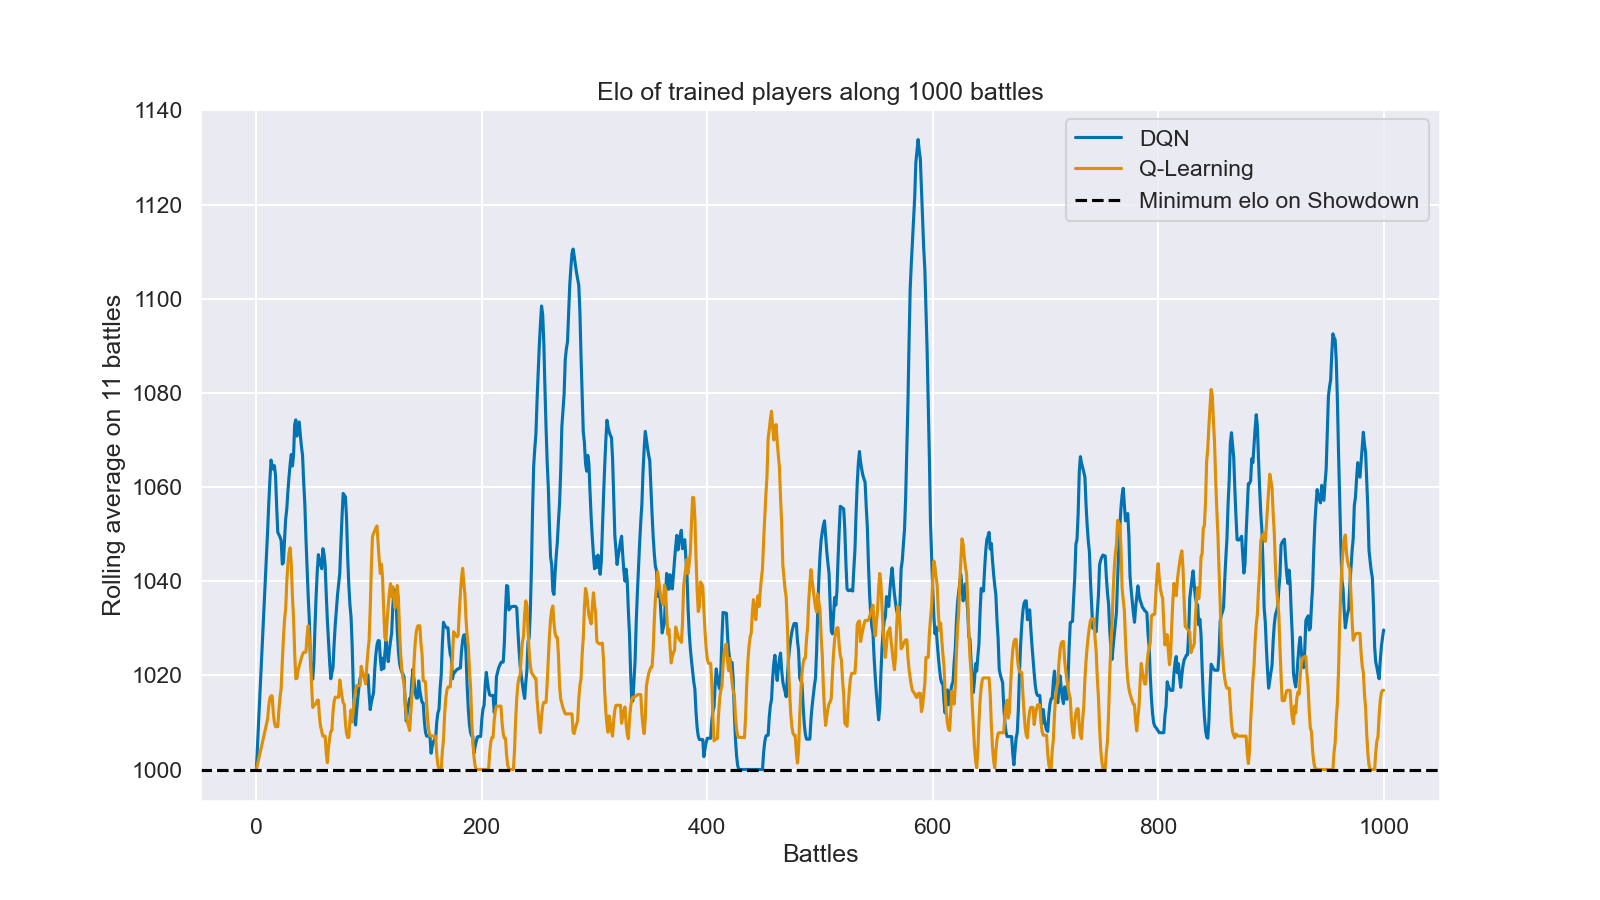
\includegraphics[width=\textwidth]{img/rank.png}
    \caption{Ladder results}
    \label{ladder_results}
\end{figure}

\begin{figure}
    \centering
    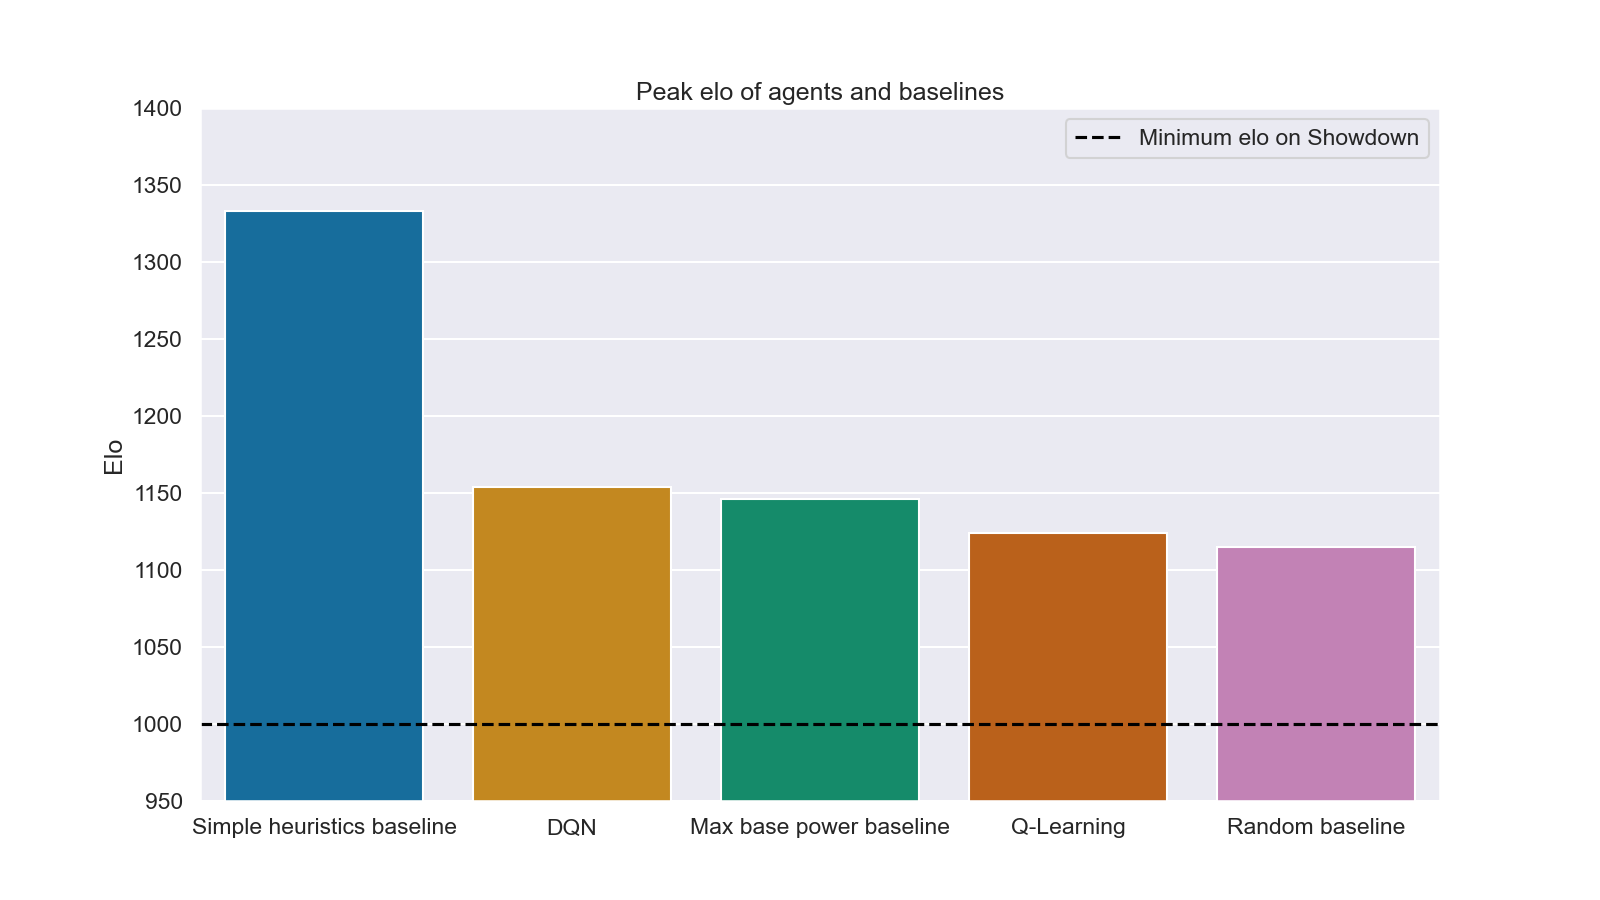
\includegraphics[width=\textwidth]{img/peak.png}
    \caption{Peak elo for trained agents and baselines}
    \label{peak_elo}
\end{figure}

\begin{figure}
    \centering
    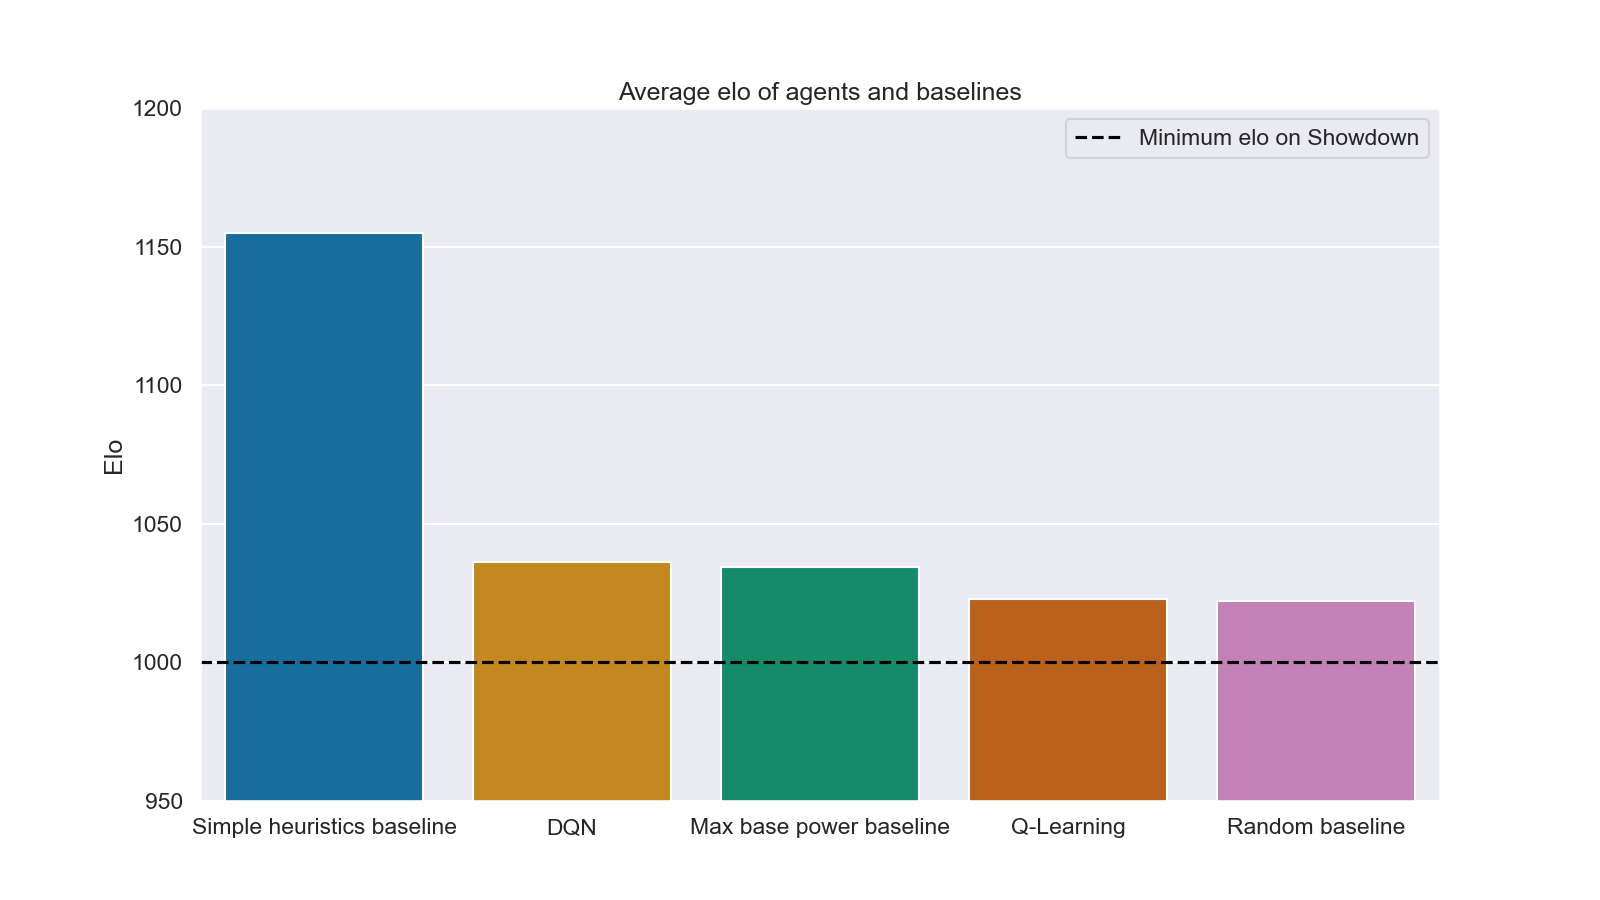
\includegraphics[width=\textwidth]{img/mean.png}
    \caption{Average elo for trained agents and baselines}
    \label{avg_elo}
\end{figure}

\section{Where to improve}

In order to obtain better results there are different angles:
\begin{itemize}
    \item use a more advanced learning algorithm, like C51 or REINFORCE;
    \item use a more complex neural network;
    \item improve the encoding of the environment to simplify the learning process;
    \item increase the number of training steps for more complex neural networks.
\end{itemize}

\clearpage

\printbibliography

\end{document}